\titreTD{\thenumTD}{Orbitales Mol\'eculaire, combinaison d'Orbitales Atomiques}

\parbox{0.5\textwidth}{\textit{Dans une mol\'ecule A$-$B, l'axe internucl\'eaire 
d\'efinit l'axe $Oz$, selon la figure du rep\`ere~:}}
\parbox{0.5\textwidth}{\centerline{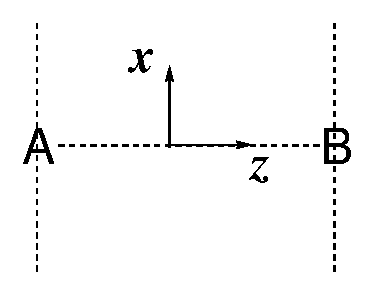
\includegraphics[scale=0.4]{figure/AB_repere.eps}}}

\exo{Principe de construction des diagrammes d'OM}
En reprenant les r\'esultats de l'exercice sur le recouvrement, page~\pageref{exo_s}, 
si le recouvrement est non-nul, pr\'ecisez et dessinez les
orbitales mol\'eculaires qui en r\'esultent. Pr\'ecisez la nature
liante ou antiliante, $\sigma$ ou $\pi$ de l'orbitale mol\'eculaire.

\vspace{0.3cm}

\begin{minipage}{4cm}
\begin{enumerate}[\bf 1)]
\item $+2p_{x\textsc{a}}\ \, |+\,2p_{x\textsc{b}}$
\item $+2p_{z\textsc{a}}\ \, |-\,2p_{z\textsc{b}}$
\item $\ \, +2s_\textsc{a}\ \, |+\,2s_\textsc{b}$
\item $\ \, +2s_\textsc{a}\ \, |+\,2p_{z\textsc{b}}$
\item $+2p_{x\textsc{a}}\ \, |+\,2s_\textsc{b}$
\end{enumerate}
\end{minipage}%
%
%\vspace{0.3cm}
\begin{minipage}{5cm}
\textbf{Exemple :}  $+2s_\textsc{a}$ et $-2s_\textsc{b}$

$c_\textsc{a}$ et $c_\textsc{b}$ sont r\'eels positifs~:

\begin{tabular}{ll}
OM liante ($\sigma$)~: &
$\sigma =  c_\textsc{a} (2s_\textsc{a}) + c_\textsc{b}(2s_\textsc{b})$ \\
& 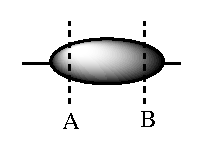
\includegraphics[width=2.0cm]{figure/sigma.eps} \\[0.5cm]
OM antiliante ($\sigma^*$)~: &
$\sigma^* = c_\textsc{a} (2s_\textsc{a}) - c_\textsc{b}(2s_\textsc{b})$ \\
& 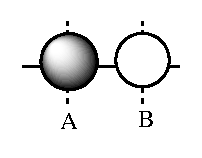
\includegraphics[width=2.0cm]{figure/sigma_star.eps} \\
\end{tabular}
\end{minipage}

%On consid\`ere l'interaction entre orbitales atomiques de deux atomes (A) et (B) formant une mol\'ecule A$-$B.
%\begin{enumerate}[~~I.]
%\item  $(1s_{A})$   et $(1s_{B})$ 
%\item  $(2p_{x_A}, 2p_{z_A})$   et $(2p_{x_B},2p_{z_B})$ 
%\item  $(2s_{A},2p_{x_A}, 2p_{y_A})$ et $(2s_{B},2p_{x_B},2p_{y_B})$
%%\item   $(2s_{A}, 3d_{z^2\textsc{A}})$   et $(2s_{B},3d_{z^2\textsc{B}})$ 
%\end{enumerate}
%Pour chacun de ces  syst\`emes  ($\textsc{I}$, $\textsc{II}$ et $\textsc{III}$), 
%repr\'esentez sur un diagramme d'\'energie le r\'esultat de l'interaction entre paires d'OA. 
%Le cas \'ech\'eant, justifiez la d\'eg\'en\'erescence de certaines  OM. 
%Pr\'ecisez pour chaque orbitale si elle est de type $\sigma$ ou $\pi$ et, si elle est  antiliante, 
%indiquez le par une * (exemple $\sigma_1^*$).\\
%
%\textit{On supposera que les OA non d\'eg\'en\'er\'ees sont suffisamment \'eloign\'ees \'energ\'etiquement pour pouvoir n\'egliger leurs interactions mutuelles~: on se limite donc \`a des interactions \`a 2 orbitales.}\\
%%--------------------------------------------------------------------------
\exo{Diagrammes d'OM \`a deux orbitales}
\textsl{Vous ne pourrez pas répondre à la question sans construire les diagrammes d'orbitales moléculaires des molécules
considérées.}\\
Pour H$_2^+$, H$_2$, He$_2^+$ et He$_2$, les \'energies de liaison sont respectivement de 255, 429, 243 et 0 kJ.mol$^{-1}$. 
Comment peut-on rendre compte qualitativement de ces valeurs dans le cadre de la th\'eorie des orbitales mol\'eculaires~?
%--------------------------------------------------------------------------
\exo{Diagramme d'une diatomique: O$_2$}
Soit l'atome d'oxyg\`ene O ($Z=8$). Ses orbitales atomiques de valence ont pour \'energies $E_{2s}=-32.4$~eV et $E_{2p}=-15.9$~eV.
\begin{enumerate}[\bf 1)]
\item \'Ecrire sa configuration \'electronique atomique dans son \'etat fondamental.
\item Quelles sont les couples d'orbitales atomiques qui vont participer \`a la formation de liaisons de type $\sigma$, de type $\pi$~?
\item Tracez le diagramme d'interaction des orbitales atomiques et y placer les 12 \'electrons de valence de la mol\'ecule. 
\item Donnez une repr\'esentation sch\'ematique des orbitales mol\'eculaires $\sigma$ et $\pi$ en insistant sur leurs diff\'erences et leurs caract\'eristiques. 
\item \'Ecrivez la configuration \'electronique mol\'eculaire (de valence) de O$_2$. 
%\item Faites figurer sur un sch\'ema le recouvrement des orbitales atomiques correspondant au dernier niveau occup\'e dans l'\'etat fondamental. S'agit-il d'un recouvrement liant ou anti-liant~?
\end{enumerate}
\clearpage
%--------------------------------------------------------------------------
\exo{Utilisation des diagrammes d'interaction}
La distance entre les atomes d'une mol\'ecule peut varier sensiblement avec la charge de l'esp\`ece.
Quelques distances internucl\'eaires sont indiqu\'ees ci-dessous pour O$_2$ et ses ions.
\begin{tabbing}
\hspace{1cm}O$_2^+$ : 1,123~\AA ; O$_2$: 1,207~\AA ; O$_2^-$: 1,300~\AA ; O$_2^{2-}$: 1,490~\AA
\end{tabbing}
On cherche \`a  expliquer la variation des distances internucl\'eaires dans la s\'erie 
en utilisant les diagrammes d'interaction. %, et les indices (ou ordres) de liaison.\\ 
Pour chaque cas vous pr\'eciserez le nombre d'\'electrons de valence, remplirez le diagramme, 
\'ecrirez  la configuration \'electronique et calculerez l'indice (ou ordre) de
liaison. Si des esp\`eces sont paramagn\'etiques le pr\'eciser (en justifiant).\\

\textit{Les trames des diagrammes sont donn\'ees ci-apr\`es.}
%--------------------------------------------------------------------------
\exo{Cas des mol\'ecules h\'et\'eronucl\'eaires~: H$-$F}
Pour la mol\'ecule HF 
($E_{1s}(\textrm{H})=-13\textrm{,}6$~eV~; $E_{2s}(\textrm{F})=-40,1$~eV et $E_{2p}(\textrm{F})=-18,6$~eV)~:
\begin{enumerate}[\bf 1)]
\item d\'eterminez le nombre d'\'electrons de valence de la mol\'ecule.
\item Dessinez le diagramme des orbitales mol\'eculaires.
\item Calculez l'indice de liaison.
\item Discutez de l'existence de paramagn\'etisme ou de moment dipolaire.
\end{enumerate}
%--------------------------------------------------------------------------

%\vrule

\begin{figure}[!h]
\begin{center}
\begin{tabular}{c}
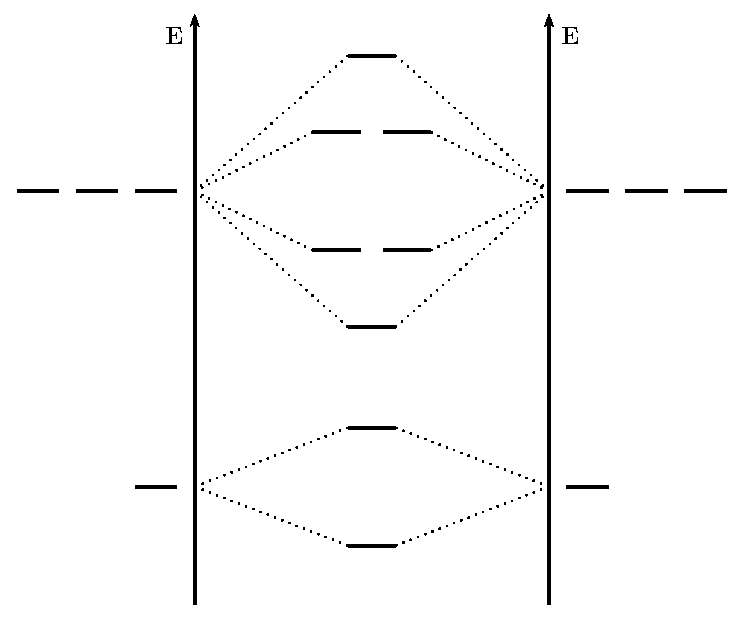
\includegraphics[height=0.4\textheight]{figure/diagOM.eps}\\[0.25cm]
\hline \\[0.25cm]
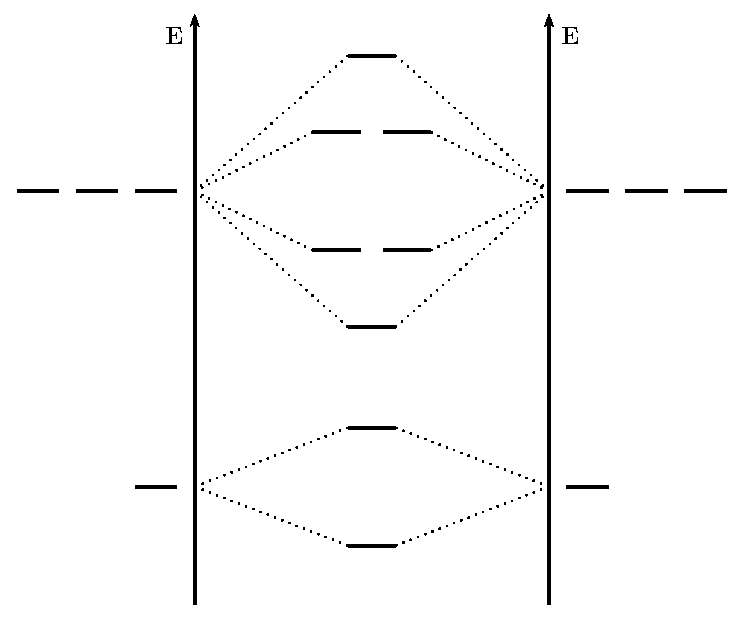
\includegraphics[height=0.4\textheight]{figure/diagOM.eps}\\
\end{tabular}
\end{center}
\end{figure}
\clearpage
%
\begin{figure}[!h]
\begin{center}
\begin{tabular}{c}
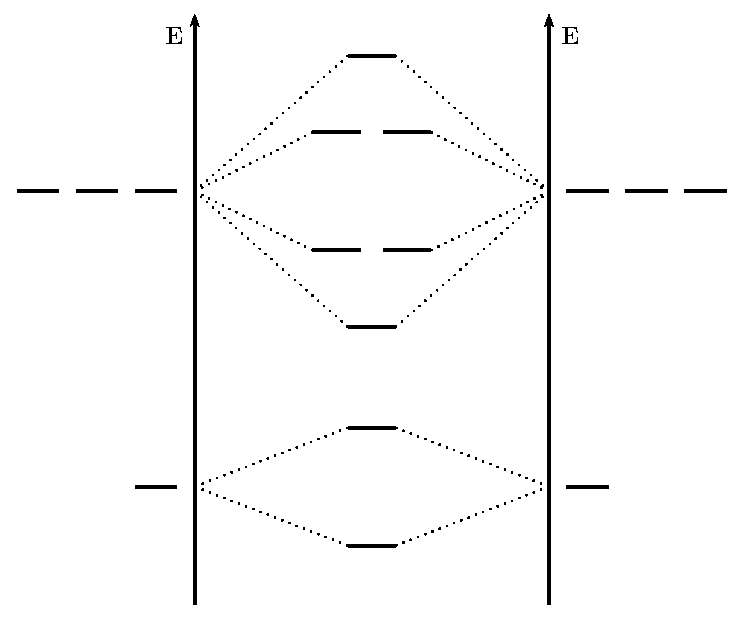
\includegraphics[height=0.4\textheight]{figure/diagOM.eps}\\[0.25cm]
\hline \\[0.25cm]
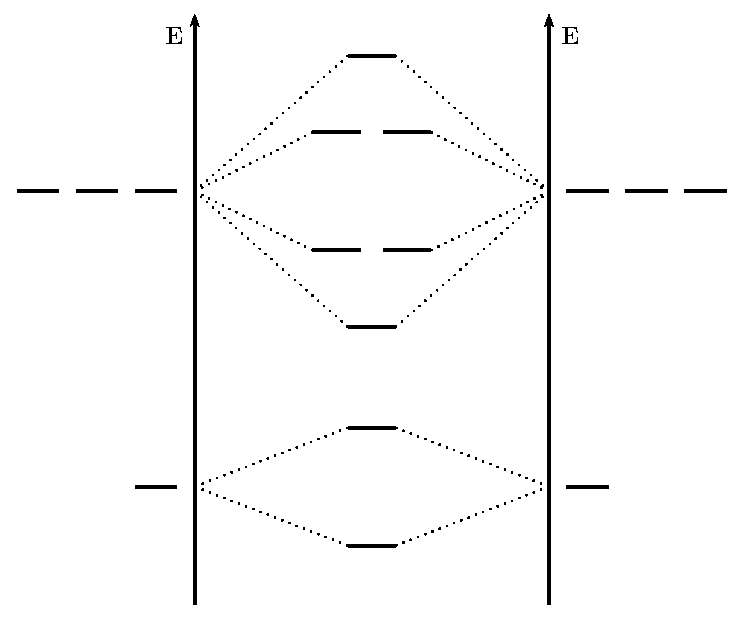
\includegraphics[height=0.4\textheight]{figure/diagOM.eps}\\
\end{tabular}
\end{center}
\end{figure}
\clearpage
